\documentclass[a4paper, 14pt]{extarticle}
\usepackage{float}
% Поля
%--------------------------------------
\usepackage{geometry}
\geometry{a4paper,tmargin=2cm,bmargin=2cm,lmargin=3cm,rmargin=1cm}
%--------------------------------------


%Russian-specific packages
%--------------------------------------
\usepackage[T2A]{fontenc}
\usepackage[utf8]{inputenc}
\usepackage[english, main=russian]{babel}
%--------------------------------------

\usepackage{textcomp}

% Красная строка
%--------------------------------------
\usepackage{indentfirst}
%--------------------------------------


%Graphics
%--------------------------------------
\usepackage{graphicx}
\graphicspath{ {./images/} }
\usepackage{wrapfig}
%--------------------------------------

% Полуторный интервал
%--------------------------------------
\linespread{1.3}
%--------------------------------------

%Выравнивание и переносы
%--------------------------------------
% Избавляемся от переполнений
\sloppy
% Запрещаем разрыв страницы после первой строки абзаца
\clubpenalty=10000
% Запрещаем разрыв страницы после последней строки абзаца
\widowpenalty=10000
%--------------------------------------

%Списки
\usepackage{enumitem}

%Подписи
\usepackage{caption}

%Гиперссылки
\usepackage{hyperref}

\hypersetup {
	unicode=true
}

%Рисунки
%--------------------------------------
\DeclareCaptionLabelSeparator*{emdash}{~--- }
\captionsetup[figure]{labelsep=emdash,font=onehalfspacing,position=bottom}
%--------------------------------------

\usepackage{tempora}

%Листинги
%--------------------------------------
\usepackage{listings}
\lstset{
  basicstyle=\ttfamily\footnotesize,
  %basicstyle=\footnotesize\AnkaCoder,        % the size of the fonts that are used for the code
  breakatwhitespace=false,        % sets if automatic breaks shoulbd only happen at whitespace
  breaklines=true,                 % sets automatic line breaking
  captionpos=t,                    % sets the caption-position to bottom
  inputencoding=utf8,
  frame=single,                    % adds a frame around the code
  keepspaces=true,                 % keeps spaces in text, useful for keeping indentation of code (possibly needs columns=flexible)
  keywordstyle=\bf,       % keyword style
  numbers=left,                    % where to put the line-numbers; possible values are (none, left, right)
  numbersep=5pt,                   % how far the line-numbers are from the code
  xleftmargin=25pt,
  xrightmargin=25pt,
  showspaces=false,                % show spaces everywhere adding particular underscores; it overrides 'showstringspaces'
  showstringspaces=false,          % underline spaces within strings only
  showtabs=false,                  % show tabs within strings adding particular underscores
  stepnumber=1,                    % the step between two line-numbers. If it's 1, each line will be numbered
  tabsize=2,                       % sets default tabsize to 8 spaces
  title=\lstname                   % show the filename of files included with \lstinputlisting; also try caption instead of title
}
%--------------------------------------

%%% Математические пакеты %%%
%--------------------------------------
\usepackage{amsthm,amsfonts,amsmath,amssymb,amscd}  % Математические дополнения от AMS
\usepackage{mathtools}                              % Добавляет окружение multlined
\usepackage[perpage]{footmisc}
%--------------------------------------

%--------------------------------------
%			НАЧАЛО ДОКУМЕНТА
%--------------------------------------

\begin{document}

%--------------------------------------
%			ТИТУЛЬНЫЙ ЛИСТ
%--------------------------------------
\begin{titlepage}
\thispagestyle{empty}
\newpage


%Шапка титульного листа
%--------------------------------------
\vspace*{-60pt}
\hspace{-65pt}
\begin{minipage}{0.3\textwidth}
\hspace*{-20pt}\centering

\includegraphics[width=\textwidth]{emblem}
\end{minipage}
\begin{minipage}{0.67\textwidth}\small \textbf{
\vspace*{-0.7ex}
\hspace*{-6pt}\centerline{Министерство науки и высшего образования Российской Федерации}
\vspace*{-0.7ex}
\centerline{Федеральное государственное бюджетное образовательное учреждение }
\vspace*{-0.7ex}
\centerline{высшего образования}
\vspace*{-0.7ex}
\centerline{<<Московский государственный технический университет}
\vspace*{-0.7ex}
\centerline{имени Н.Э. Баумана}
\vspace*{-0.7ex}
\centerline{(национальный исследовательский университет)>>}
\vspace*{-0.7ex}
\centerline{(МГТУ им. Н.Э. Баумана)}}
\end{minipage}
%--------------------------------------

%Полосы
%--------------------------------------
\vspace{-25pt}
\hspace{-35pt}\rule{\textwidth}{2.3pt}

\vspace*{-20.3pt}
\hspace{-35pt}\rule{\textwidth}{0.4pt}
%--------------------------------------

\vspace{1.5ex}
\hspace{-35pt} \noindent \small ФАКУЛЬТЕТ\hspace{80pt} <<Информатика и системы управления>>

\vspace*{-16pt}
\hspace{47pt}\rule{0.83\textwidth}{0.4pt}

\vspace{0.5ex}
\hspace{-35pt} \noindent \small КАФЕДРА\hspace{50pt} <<Теоретическая информатика и компьютерные технологии>>

\vspace*{-16pt}
\hspace{30pt}\rule{0.866\textwidth}{0.4pt}

\vspace{11em}

\begin{center}
\Large {\bf Лабораторная работа № 6} \\
\large {\bf по курсу <<Численные методы линейной алгебры>>} \\
\large <<Изучение скорости сходимости
однопараметрического метода>>
\end{center}\normalsize

\vspace{8em}


\begin{flushright}
  {Студент группы ИУ9-71Б Баев Д.А \hspace*{15pt}\\
  \vspace{2ex}
  Преподаватель Посевин Д. П.\hspace*{15pt}}
\end{flushright}

\bigskip

\vfill


\begin{center}
\textsl{Москва 2023}
\end{center}
\end{titlepage}
%--------------------------------------
%		КОНЕЦ ТИТУЛЬНОГО ЛИСТА
%--------------------------------------

\renewcommand{\ttdefault}{pcr}

\setlength{\tabcolsep}{3pt}
\newpage
\setcounter{page}{2}

\section{Задание}\label{Sect::task}
1. Реализовать однопараметрический метод для положительной симметричной матрицы
произвольного размера N × N.

2. Вычислить спектр матрицы A методом Крылова или Данилевского, которые были
реализованы ранее, и получить минимальное и максимальное значение спектра λmin и
λmax. После чего вычислить $τ_{\text{опт}$ = 2/($λ_{\text{min}$ +$λ_{\text{max}$).

3. Построить график зависимости количества итераций n решения уравнения A·x=f
однопараметрическим методом в зависимости от значения τ лежащего в пределах от 0 до
2/ $λ_{\text{max}$. Определить τопт из графика и сравнить с теоретическим значением полученным в
пункте 2.

4. Для каждого эксперимента пункта 3 вывести условие сходимости. Решение системы для оценки неравенства приведенного выше
можно получить путем решения A·x=f методом Гаусса. Другими словами требуется убедиться в том, что выполняются условия теоремы о сходимости
однопараметрического метода. Обязательно, дополнительно проверить и показать,
что для каждого k модуль максимального значения $λ_{\text{i}$ меньше 1.

\newpage
\section{Исходный код}

Исходный код программы представлен в листингах~\ref{lst:code1}--~\ref{lst:code2}.

\begin{figure}[H]
\begin{lstlisting}[language={},caption={Реализация однопараметрического метода со всеми необходимыми проверками},label={lst:code1}]
def single_parameter(A, b, tao, spectre, delta=1e-7):
    n = len(A)
    P = np.eye(n) - tao * A
    g = tao * b

    x_gauss = np.linalg.solve(A, b)
    Mu = np.array([1 - tao * spectre[i] for i in range(n)])
    assert np.max(np.abs(Mu)) < 1
    k = 0
    x_prev = np.zeros(shape=(n, ))
    difference = np.array([1] * n)
    x_k = None
    while norm(difference) > delta:
        x_k = mul_matrix_by_vector(P, x_prev) + g
        difference = x_k - x_prev
        r = x_k - x_gauss
        #if (norm(r) ** 2) > max(Mu[i] ** 2 for i in range(n)) * norm(x_prev - x_gauss) ** 2:
        #    print("One", norm(r) ** 2)
        #    print("Two", max(Mu[i] ** 2 for i in range(n)) * norm(x_prev - x_gauss) ** 2)
        if np.round(norm(r) ** 2, 7) > np.round(max(Mu[i] ** 2 for i in range(n)) * norm(x_prev - x_gauss) ** 2, 7):
            print(f"Proverka is not okay: tao - {tao}, iter = {k}")
            #return None, 0
        x_prev = deepcopy(x_k)
        k += 1
    return x_k, k
\end{lstlisting}
\end{figure}

\begin{figure}[H]
\begin{lstlisting}[language={},caption={Получение результатов и построение графика количества итераций от значения параметра},label={lst:code2}]
def get_tao_plot(n):
    A = generate_sim_matrix(n=n, diag=1)
    x = np.random.uniform(0, 10, size=(n, ))
    b = mul_matrix_by_vector(A, x)


    spectre = eig(A)

    lambda_min, lambda_max = min(spectre), max(spectre)
    assert lambda_min > 0

    tao_opt = 2 / (lambda_min + lambda_max)
    _, iter_opt = single_parameter(A, b, tao_opt, spectre)
    print(f"Analytical solution tao_opt: {tao_opt}")
    print(f"Optimal iterations: {iter_opt}")
    tao_array = np.linspace(0, 2 / lambda_max, 100, True)
    tao_array = tao_array[1:-1]
    iters_array = []

    for tao in tao_array:
        _, i = single_parameter(A, b, tao, spectre)
        iters_array.append(i)

    i_exp = np.argmin(iters_array)
    plt.plot(tao_array, iters_array)
    plt.scatter(tao_opt, iter_opt, color="red")
    plt.scatter(tao_array[i_exp], iters_array[i_exp])
    print(f"Experiment solution tao_opt: {tao_array[i_exp]}")
    print(f"Optimal iterations: {iters_array[i_exp]}")
\end{lstlisting}
\end{figure}



\section{Результаты}

Результаты поиска оптимального значения метода и исследования количества итераций от значений параметра приведены на рисунках~\ref{fig:img1}-~\ref{fig:img3}.


\begin{figure}[H]
\centering
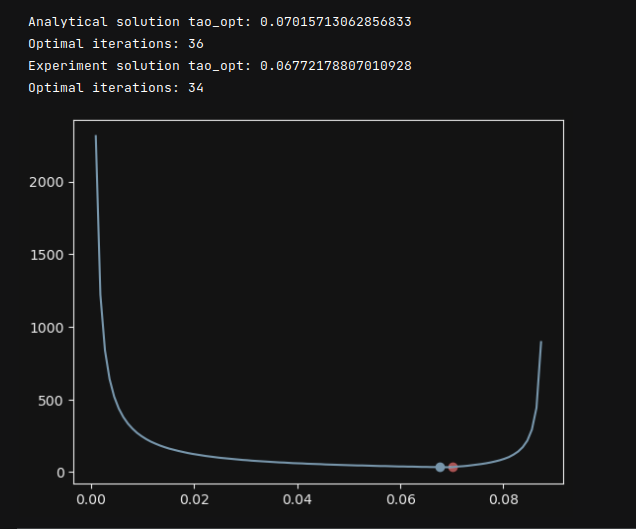
\includegraphics[width=0.8\textwidth]{images/res1.png}
\caption{График зависимости количества итераций от значения параметра в области сходимости метода для матрицы 4x4}
\label{fig:img1}
\end{figure}


\begin{figure}[H]
\centering
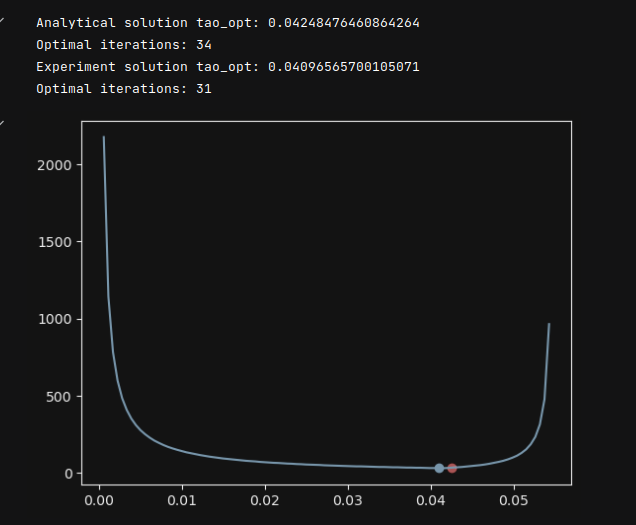
\includegraphics[width=0.8\textwidth]{images/res2.png}
\caption{График зависимости количества итераций от значения параметра в области сходимости метода для матрицы 7x7}
\label{fig:img2}
\end{figure}


\begin{figure}[H]
\centering
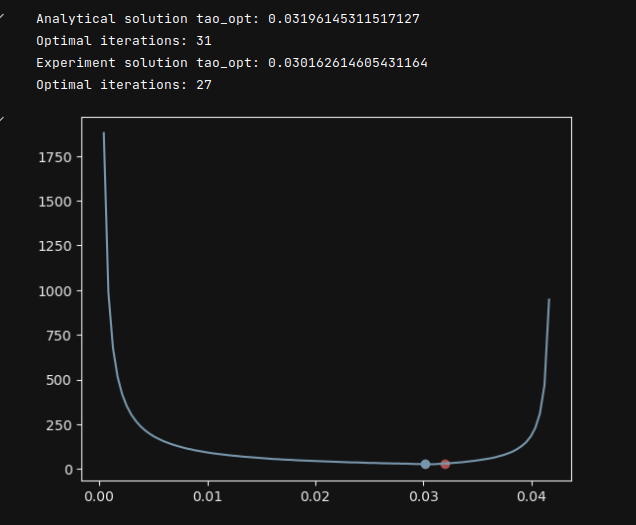
\includegraphics[width=0.8\textwidth]{images/res3.png}
\caption{График зависимости количества итераций от значения параметра в области сходимости метода для матрицы 10x10}
\label{fig:img3}
\end{figure}


\section{Выводы}
В результате выполения лабораторной работы был реализован однопараметрический метод решения СЛАУ с матрицей коофициентов NxN. В процессе была исследована скорость сходимости метода, а также определены аналитические и эксперементальные оптимальные значения параметра. Также было исследовано условие сходимости метода на каждой его итерации. Стоит заметить, что в практических условиях при значениях параметра, больших чем оптимальное, данное условие будет выполняться не всегда, ввиду неточности вычислений на ЭВМ. Данная проблема решается округлением
\end{document}